\documentclass[12pt]{article}
\usepackage[utf8]{inputenc}
\usepackage{style}

\title{Oracle Quantum Computing}
\author{Joshua Spayd}
\date{\today}

\begin{document}
\maketitle

\section{Introduction}
It is the objective of the theoretical sciences to develop mathematical models
that describe natural phenomena, and when faced with a result that contradicts
existing models, it is the responsibility of the theorist to augment these
models to reconcile with the observed phenomena, and to resolve
inconsistencies across scientific theories. The strong Church-Turing thesis
conjectures that every physically realizable computation model can be
simulated by a Turing machine with polynomial overhead in runtime, but
physicist Richard Feynman \cite{Fey82} notes that the obvious classical
algorithm for simulating a quantum system of $n$ particles runs exponentially
in $n$ and suggests that computers be equipped with quantum mechanical gates
in order to enable efficient simulation of quantum systems. If quantum systems
cannot be efficiently simulated by Turing machines --- and if general-purpose
quantum computers are physically realizable --- then the strong Church-Turing
thesis is false, and we require a new model of computation. Though questions
of the feasibility and relative efficiency of quantum computers are yet
unanswered, this uncertainty has not prevented theorists from developing
quantum computational models. In this paper, we will formalize quantum computing
and quantum oracles, and then we will describe a few results from quantum
complexity theory, with emphasis on the result from \cite{BB92a} that relative to
certain oracles, quantum computers are more powerful than nondeterministic
computers, or in the words of  Berthiaume and Brassard, that ``quantum can beat
nondeterminism.''


\section{Quantum superposition: the two-slit experiment}
Before we attempt to formalize quantum computation, it will help to understand
the physical ideas behind such a formalization. To illustrate these principles,
we turn to the two-slit experiment. In the two-slit experiment, a photon source
id placed on one side of a wall that has two slits in it. On the other side is
an array of detectors that light up when hit by a photon. Consider the rate at
which photons hit these detectors. If one slit is covered, we might expect that
the detector behind the open slit will receive the highest rate of photons per
hour, which is indeed what happens, as depicted in \cref{fig:two-slit-1}.

\begin{figure}[H]
  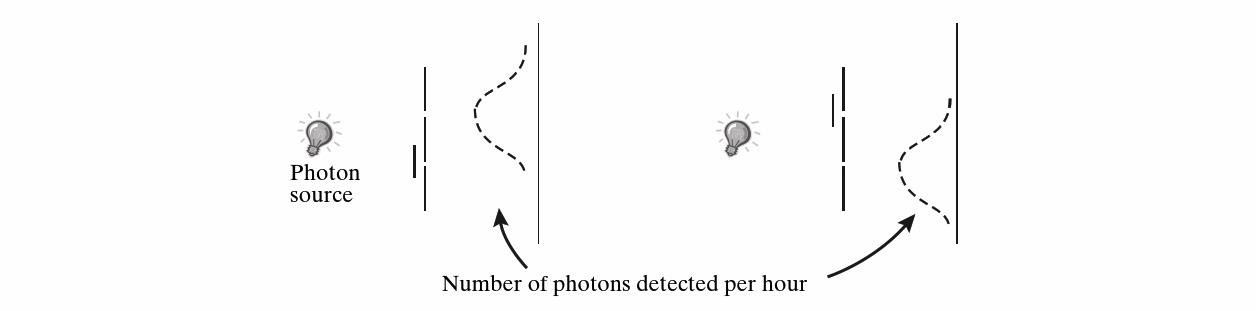
\includegraphics[width=\textwidth]{two-slit-1}
  \caption{\cite[p. 203]{AB09}}
  \label{fig:two-slit-1}
\end{figure}

If we uncover both slits, then we may expect that a detector will receive a rate
of photons equal to the sum of the rates it receives when one of each of the
slits is covered, but this is not what happens. In fact, as depicted in
\cref{fig:two-slit-2}, some detectors even receive a lower rate of photons than
this sum.

\begin{figure}[H]
  
\includegraphics[width=\textwidth]{two-slit-2}
  \caption{\cite[p. 203]{AB09}}
  \label{fig:two-slit-2}
\end{figure}

This phenomenon can only be explained by quantum mechanics. When a photon leaves
the photon source, it does not follow a single path to some detector; rather, it
instantaneously explores all possible paths, where each path has some associated
\emph{amplitude}, which may be positive or negative (or zero). If two paths
arrive at the same detector with opposite signs, then they cancel-out, or
\emph{interfere}. However, perhaps we are skeptical of this all-paths
exploration, and we decide to add detectors at each slit that light up when a
photon passes through the slit. If photons are truly exploring all possible
paths, then we might expect to measure some of the same photons at both slits.
But now that we are measuring the photons at the slits, we instead see what we
originally expected: each detector receives a rate of photons equal to the
sum of the rates of photons it receives when one of each of the slits is
covered. This experiment gives us an idea of both some of the strengths and
weaknesses of quantum computers: if we can in some sense ``explore all paths,''
then we may be able to simulate nondeterminism efficiently, but the nature of
our quantum parallelism must play nicely with quantum interference, and once we
measure a result, we lose any parallelism that we may have.


\section{Modeling quantum computation}
We begin our model with a description of memory. On a classical computer, we
normally model memory as a sequence of bits, each of which can be 0 or 1. In
our model of quantum computers, the smallest piece of memory is the
\emph{qubit}, which can take on the basic states $\qz$ and $\qo$, or may also be
in a \emph{superposition} of these states of the form
$$
  \alpha_0\qz + \alpha_1\qo,
$$
where $\alpha_0, \alpha_1 \in \CC$ are \emph{amplitudes} satisfying
$\abs*{\alpha_0}^2 + \abs*{\alpha_1}^2 = 1$.\footnote{Recall that for a complex
number $z = a + bi$ where $i=\sqrt{-1}$, we have $\abs*{z} = \sqrt{a^2+b^2}$.}
When we observe the qubit, it is revealed to be in state $\qz$ with probability
$\abs*{\alpha_0}^2$ and state $\qo$ with probability $\abs*{\alpha_1}^2$. Once
the qubit is measured, its amplitude wave \emph{collapses}, and the values of
its amplitudes are lost. Our state of memory, then, is an $m$-qubit register
$\reg*{b_1, b_2, \dots, b_m}$ described by a superposition of the form
$$
  \alpha_{0\dots 0}\reg*{0\dots 0}
  + \alpha_{0\dots 1}\reg*{0\dots 1}
  + \dots
  + \alpha_{1\dots 1} \reg*{1\dots 1},
$$
where $\sum_{x \in \zo^m} \abs*{\alpha_x}^2 = 1$. When the system is observed,
it is revealed to be in state $\reg*{x}$ with probability $\abs*{\alpha_x}^2$
for each $x \in \zo^m$. We will sometimes denote the state $\reg*{xy}$ as
$\reg*{x}\reg*{y}$. It will also often be useful to think of quantum states as
vectors of amplitudes, where the amplitudes are given in the lexicographic order
of their associated basic states. For example, a 2-qubit register in the state
$$
  \alpha_{00} \reg*{00}
  + \alpha_{01} \reg*{01}
  + \alpha_{10} \reg*{10}
  + \alpha_{11} \reg*{11}
$$
can be represented by the vector $\paren*{\alpha_{00}, \alpha_{01}, \alpha_{10},
\alpha_{11}}$.

\subsection{Quantum operations}
Now that we have a model of memory, we can define the quantum operations that
act on memory.
\begin{defn}[Quantum operation {\cite[p. 210]{AB09}}]
  \label{defn:op}
  A \emph{quantum operation} for an $m$-qubit register is a funciton $F :
  \CC^{2^m} \to \CC^{2^m}$ that maps its previous state to the new state and
  satisfies the following conditions:
  \begin{adjustwidth}{0.25in}{0in}
    \emph{Linearity:} $F$ is a linear function. That is, for every $\vec{v} \in
    \CC^{2^n}$, $F(\vec{v}) = \sum_x \vec{v}_x F(\reg*{x})$. \\
    \emph{Norm preservation:} $F$ maps unit vectors to unit vectors. That is,
    for every $\vec{v}$ with $\norm*{\vec{v}}_2=1$,
    $\norm*{F(\vec{v})}_2=1$.\footnote{Here, $\norm*{\vec{v}}_2$ denotes the
    $\ell^2$ norm of $\vec{v}$, i.e. $\norm*{\vec{v}} = \sqrt{\sum_i
    \abs*{\vec{v}_i}^2}$.}
  \end{adjustwidth}
\end{defn}
The linearity condition comes from quantum mechanics, and the norm preservation
condition is natural since only unit vectors can describe states. We now
describe several specific quantum operations.
\begin{adjustwidth}{0.25in}{0in}
  \emph{Flipping qubits:} If we wish to flip the first qubit of an $m$-qubit
  register, then this can be done by mapping the basis state $\reg*{b, x}$ to
  $\reg*{1-b, x}$. Since we only modify the first qubit, we can instead use the
  shorthand $\reg*{b} \mapsto \reg*{1-b}$. Also note that because quantum
  operations are linear, it suffices to describe their actions on a basis. Thus,
  the bit flipping operation can be described as $\qz \mapsto \qo$ and $\qo
  \mapsto \qz$. \vspace{0.5\baselineskip}

  \noindent \emph{Reordering qubits:} If we wish to exchange the values of two
  qubits, it suffices to use the operation
  \begin{align*}
    \reg*{00} &\mapsto \reg*{00} \\
    \reg*{01} &\mapsto \reg*{10} \\
    \reg*{10} &\mapsto \reg*{01} \\
    \reg*{11} &\mapsto \reg*{11}.
  \end{align*}
  If we interpret quantum states as vectors, then this operation can be
  described by the matrix
  $$
    \begin{pmatrix}
      1 & 0 & 0 & 0 \\
      0 & 0 & 1 & 0 \\
      0 & 1 & 0 & 0 \\
      0 & 0 & 0 & 1
    \end{pmatrix}.
  $$ \vspace{0.5\baselineskip}

  \noindent \emph{AND of two bits:} Suppose that we want to take the AND of two
  qubits. It may be tempting to write this as $\reg*{b_1b_2} \mapsto \reg*{b_1
  \land b_2}\reg*{b_2}$, but this operation is not norm-preserving. To handle
  this, instead of writing to the first bit, we write to an additional third
  bit, which we assume starts as zero. We use the operation
  $$
    \reg*{b_1}\reg*{b_2}\reg*{b_3} \mapsto \reg*{b_1}\reg*{b_2}\reg*{b_3 \xor
    (b_1 \land b_2)},
  $$
  where $\xor$ denotes the XOR operation. We can also describe this operation
  with the matrix
  $$
    \begin{pmatrix}
      1 & 0 & 0 & 0 & 0 & 0 & 0 & 0 \\
      0 & 1 & 0 & 0 & 0 & 0 & 0 & 0 \\
      0 & 0 & 1 & 0 & 0 & 0 & 0 & 0 \\
      0 & 0 & 0 & 1 & 0 & 0 & 0 & 0 \\
      0 & 0 & 0 & 0 & 1 & 0 & 0 & 0 \\
      0 & 0 & 0 & 0 & 0 & 1 & 0 & 0 \\
      0 & 0 & 0 & 0 & 0 & 0 & 0 & 1 \\
      0 & 0 & 0 & 0 & 0 & 0 & 1 & 0
    \end{pmatrix}.
  $$
  This operation is known as the \emph{Toffoli gate}. It is also possible to
  obtain a quantum OR operation. \vspace{0.5\baselineskip}

  \noindent \emph{The Hadamard operation:} Thus far, we have only seen
  operations that permute amplitudes, but we are not restricted to such
  operations. One operation that does otherwise is the \emph{Hadamard}
  operation, which can be described by the mapping
  \begin{align*}
    \qz &\mapsto \frac{1}{\sqrt{2}} \qz + \frac{1}{\sqrt{2}} \qo \\
    \qo &\mapsto \frac{1}{\sqrt{2}} \qz - \frac{1}{\sqrt{2}} \qo,
  \end{align*}
  or by the matrix
  $$
    \frac{1}{\sqrt{2}} \begin{pmatrix}
      1 & 1 \\
      1 & -1
    \end{pmatrix}.
  $$
\end{adjustwidth}

\subsection{Quantum Turing machines and the class $\BQP$}
Applying many operations to the entirety of a quantum register may not be
feasible, so we define quantum computation using local operations: operations
that act on a finite number of qubits. We call these operations
\emph{elementary}.
\begin{defn}[Elementary quantum operations or quantum gates {\cite[p.
             213]{AB09}}]
  A quantum operation is called \emph{elementary}, or sometimes a \emph{quantum
  gate}, if it acts on three or fewer qubits of the register.
\end{defn}
To describe an elementary operation, it suffices to describe three qubit
positions and a matrix. With elementary quantum operations defined, we have all
we need to define quantum computation and $\BQP$, the quantum analog of $\PP$ or
$\BPP$.

\begin{defn}[Quantum computation and the class $\BQP$ {\cite[p. 213]{AB09}}]
  \label{defn:bqp}
  Let $f : \zo^* \to \zo$ and $T : \NN \to \NN$ be some functions. We say that
  $f$ is \emph{computable in quantum $T(n)$-time} if there is a polynomial-time
  classical TM that on input $\paren*{1^n, 1^{T(n)}}$ for any $n \in \NN$
  outputs the descriptions of quantum gates $F_1, \dots, F_T$ such that for
  every $x\in \zo^n$, we can compute $f(x)$ with probability at least
  $\nfrac{2}{3}$ by the following process:
  \begin{enumerate}
    \item Initialize an $m$-qubit quantum register to the state
      $\reg*{x0^{n-m}}$ (i.e., $x$ padded with zeroes), where $m \le T(n)$.
    \item Apply ons after the other $T(n)$ elementary quantum operations $F_1,
      \dots, F_T$ to the register.
    \item Measure the register and let $Y$ denote the obtained value. (That is,
      if $\vec{v}$ is the final state of the register, then $Y$ is a random
      variable that takes the value $y$ with probability $\abs*{\vec{v}_y}^2$
      for every $y \in \zo^m$.)
    \item Output $Y_1$.
  \end{enumerate}
  A Boolean function $F : \zo^* \to \zo$ is in $\BQP$ if there is some
  polynomial $p : \NN \to \NN$ such that $f$ is computable in quantum
  $p(n)$-time.
\end{defn}

Given our quantum analogs of the AND and OR operations, along with the inherent
randomness built into $\BQP$, the following result should be unsurprising.

\begin{thm}
  \label{thm:bpp-bqp}
  $\BPP \subseteq \BQP$.
\end{thm}

For a proof of \cref{thm:bpp-bqp}, see page 215 of \cite{AB09}. The above
theorem gives us a decent lower bound on the power of $\BQP$. We do not have
much of an upper bound on the power of $\BQP$, but we do know that $\BQP$ is not
infinitely powerful.

\begin{thm}
  \label{thm:bqp-pspace}
  $\BQP \subseteq \PSPACE$.
\end{thm}

A proof of \cref{thm:bqp-pspace}, see page 230 of \cite{AB09}. Most people,
however, believe that $\BQP$ is not as powerful as $\NP$.

\begin{conj}
  \label{conj:np-bqp}
  $\NP \not\subseteq \BQP$.
\end{conj}

Perhaps the most compelling evidence for this is the following result.

\begin{thm}[\cite{BBBV97}]
  \label{thm:no-black-box}
  Relative to an oracle chosen uniformy at random, with probability 1, the class
  $\NP$ cannot be solved on a quantum Turing machine in time $\smallo{2^{n/2}}$.
\end{thm}

The interpretation given in \cite{BBBV97} of this result is that ``there is no
black-box approach to solving $\NP$-complete problems using some uniquely
quantum features of QTMs.'' Still, there is evidence that quantum computers have
at least some more power than classical computers.

\begin{conj}
  $\BPP \subsetneq \BQP$.
\end{conj}

This is supported by the fact that there is a polynomial-time quantum algorithm
for factoring integers.

\begin{thm}[\cite{Sho97}]
  \label{thm:shor}
  $\lang{Factoring} \in \BQP$.
\end{thm}

\Cref{thm:shor} is interesting not only because there is no known
polynomial-time randomized algorithm for $\lang{Factoring}$, but also because
many cryptosystems rely on $\lang{Factoring}$ being hard. If quantum computers
become reliable and common enough, then those cryptosystems will no longer be
secure. Readers curious about Shor's algorithm can of course refer to
\cite{Sho97}, but may find the explanation beginning on page 221 of \cite{AB09}
easier to follow.

Given \cref{conj:np-bqp} and \cref{thm:no-black-box}, the following result may
be surprising.

\begin{thm}[\cite{BB92a}]
  \label{thm:bqp-beat-np}
  There exists an oracle relative to which there is a set that can be recognized
  in worst-case linear time by a quantum computer, yet any nondeterministic
  Turing machine that accepts it must take exponential time on infinitely many
  inputs.
\end{thm}
The authors of \cite{BB92a} call this ``quantum can beat nondeterminism,'' and it
is this result that we will prove in the remainder of this paper.

\section{Quantum can beat nondeterminism \cite{BB92a}}

The proof of \cref{thm:bqp-beat-np} given in \cite{BB92a} relies on a theorem
from \cite{DJ92}. Let $X \subseteq \zo^*$ be a language. We say that $B(X)$
holds if for all $n$, one of the following is true:
\begin{enumerate}[label=(\arabic*)]
  \item $X \cap \zo^n = \emptyset$ (i.e., $X$ contains no strings of length
    $n$); or
  \item $\abs*{X \cap \zo^n} = 2^{n-1}$ (i.e., $X$ contains exactly $2^{n-1}$
    strings of length $n$).
\end{enumerate}
Then the theorem is as follows.

\begin{thm}[\cite{DJ92}]
  \label{thm:promise}
  Let $X \subseteq \zo^*$ be a language such that $B(X)$ holds, and suppose that
  there is a classical algorithm that decides $X$ in time $\bigo{t(n)}$ for all
  $x$ of length $n$, where $t(n) \ge n$ for all $n$. Then a quantum computer can
  decide in worst-case time $\bigo{t(n)}$ whether or not $X$ contains any
  strings of length $n$.\footnote{Though this theorem is based on a result in
  \cite{DJ92}, this particular formulation of the result comes from
  \cite{BB92b}.}
\end{thm}

We do not prove \cref{thm:promise} here, but we recommend that curious readers
refer to \cite{DJ92}, which provides a proof that is significantly less dense
than one might expect. Our proof of \cref{thm:bqp-beat-np} proceeds by using an
enumeration of all nondeterministic Turing machines to construct a language $Y$
where $B(Y)$ holds so that with an oracle for $Y$, on input $1^n$, a quantum
computer can decide in polynomial time if $Y$ contains any strings of length
$n$, but no nondeterministic Turing machine can decide the same problem in
polynomial time.

\begin{mdframed}
\begin{proof}[Proof of \cref{thm:bqp-beat-np}]
  Let $N_1, N_2, \dots$ be a standard enumeration of all nondeterministic Turing
  machines, and let $\alpha : \NN \to \NN$ be some function such that for every
  $i \in \NN$, there are infinitely many $n \in \NN$ such that $\alpha(n) = i$.
  Finally, let $\wp : \NN \to \NN$ be defined as
  $$
    \wp(n) = \begin{cases}
              1            & \text{if $n=1$} \\
              2^{\wp(n-1)} & \text{if $n>1$}.
             \end{cases}
  $$
  We use these to construct a language $Y$ where $B(Y)$ holds. We construct $Y$
  in stages, constructing $Y_1, Y_2, \dots$ such that $Y = \bigcup_{n\ge 1}
  Y_n$. At the end of stage $n$, $Y$ will be defined for all strings of length
  less than $\wp(n+1)$. In particular, at each stage $n$, we ensure that $Y$
  contains either 0 or $2^{\wp(n)-1}$-many strings of length $\wp(n)$, and
  simultaneously that on input $1^{\wp(n)}$, any nondeterministic Turing machine
  must take more than $2^{\wp(n)-1}$ steps. We construct $Y$ as follows.
  \begin{enumerate}
    \item Initially, set $Y_1=\emptyset$.
    \item At stage $n \ge 1$, simulate every path of nondeterministic machine
      $N_{\alpha(n)}$ on input $1^{\wp(n)}$ with oracle $Y_n$ for up to
      $2^{\wp(n)-1}$ steps for each path.
      \begin{itemize}
        \item If there is a path that makes the machine exceed $2^{\wp(n)-1}$
          steps, or if the machine rejects, set $Y_{n+1}=Y_n$ and go to the next
          stage.
        \item If the machine accepts within $2^{\wp(n)-1}$ steps, select an
          arbitrary accepting path and let $Q_n$ be the set of oracle questions
          asked along that path. Because of the time bound on the computation,
          note that $Q_n$ contains no more than $2^{\wp(n)-1}$ questions, and
          none of these questions can be of length greater than $2^{\wp(n)-1}$.
          But there are $2^{\wp(n)}$ strings of length $\wp(n)$, and therefore
          we can form a set $R_n \subset \zo^{\wp(n)}$ such that $R_n \cap
          Q_n = \emptyset$ and the number of elements in $R_n$ is exactly
          $2^{\wp(n)-1}$. Let $Y_{n+1} = Y_n \cup R_n$ and go to the next stage.
      \end{itemize}
  \end{enumerate}
  Let $Y = \bigcup_{n\ge 1} Y_n$. Note that $B(Y)$ holds because we took care at
  each step of either putting nothing in $Y$, or of putting exactly half the
  strings of a given length (and we never put in strings of the same length more
  than once). Now we define the language $S_Y$ as
  $$
    S_Y = \curl*{1^n \mid
                 \mbox{$Y$ does not contain any strings of length $n$}}.
  $$
  \Cref{thm:promise} tells us that given an oracle for $Y$, a quantum computer
  can decide $S_Y$ in linear time. To complete the proof, we must now show that
  nondeterministic Turing machines must take exponential time to decide $S_Y$.
  To do so, consider an arbitrary nondeterministic Turing machine $N_i$ that
  purports to accept language $S_Y$. By definition of $\alpha$, there are
  infinitely many integers $n$ such that $i = \alpha(n)$, so $Y$ is defined in
  part based on $N_i$. For any such $n$, we claim that $N_i$ using an oracle for
  $Y$ must take more than $2^{\wp(n)-1}$ steps on input $1^{\wp(n)}$. To prove
  this claim, consider what happens when we run $N_i$ on input $1^{\wp(n)}$, but
  with an oracle for $Y_n$. We consider three cases.
  \begin{itemize}
    \item If at least one path of the computation of $N_i^{Y_n}$ on $1^{\wp(n)}$
      takes more than $2^{\wp(n)-1}$ steps, by construction, $Y_{n+1} = Y_n$ and
      therefore $Y$ and $Y_n$ agree on all strings of length smaller than
      $\wp(n+1) = 2^{\wp(n)}$. But then the first $2^{\wp(n)}$ steps of any
      computation of $N_i$ on input $1^{\wp(n)}$ are identical regardless of
      whether $Y$ or $Y_n$ is used as an oracle since the machine cannot
      formulate questions long enough to distinguish between these oracles
      within that time. Therefore, using oracle $Y$ as well, there is at least
      one path of the computation of $N_i$ on $1^{\wp(n)}$ that takes more than
      $2^{\wp(n)-1}$ steps.
    \item If $N_i^{Y_n}$ rejects $1^{\wp(n)}$ within $2^{\wp(n)-1}$ steps, then
      $Y$ and $Y_n$ agree on all strings of length smaller than $2^{\wp(n)}$
      just as in the previous case. By the same argument, $N_i$ behaves
      identically on input $1^{\wp(n)}$ regardless of whether it uses oracle $Y$
      or $Y_n$. Therefore, $N_i$ rejects $1^{\wp(n)}$ also with oracle $Y$. But
      $N_i^Y$ is assumed to recognize $S_Y$, and hence $1^{\wp(n)} \not\in S_Y$,
      which means that $Y \cap \zo^{\wp(n)} \ne \emptyset$. This is impossible
      since by construction no strings of length $\wp(n)$ are put into $Y$ in
      this case.
    \item If $N_i^{Y_n}$ accepts $1^{\wp(n)}$ within $2^{\wp(n)-1}$ steps,
      consider the accepting path used in stage $n$ of the construction of $Y$.
      The set $R_N$ is designed so that is contains none of the oracle questions
      asked along this path. Since $Y_n$ and $Y$ differ on strings of length
      smaller than $2^{\wp(n)}$ only in that the strings in $R_n$ belong to $Y$
      but not to $Y_n$, the same accepting path of $N_i$ on $1^{\wp(n)}$ exists
      when an oracle for $Y$ is used. Although $N_i^Y$ and $N_i^{Y_n}$ could
      behave differently on all other paths, one accepting path is enough for a
      nondeterministic machine to accept, and therefore $N_i^Y$ accepts
      $1^{\wp(n)}$. But again $N_i^Y$ is assumed to recognize $S_Y$, and hence
      $1^{\wp(n)} \in S_Y$, which means that $Y \cap \zo^{\wp(n)} = \emptyset$.
      This is impossible since by construction $2^{\wp(n)-1}$ strings of length
      $\wp(n)$ are put into $Y$ in this case.
  \end{itemize}
  Only the first case remains possible, and thus by Sherlock Holmes' principle
  it is the truth. But that case implies that $N_i^Y$ on $1^{\wp(n)}$ takes more
  than $2^{\wp(n)-1}$ steps on at least one of its computation paths. Since this
  occurs for infinitely many values of $n$, any nondeterministic Turing machine
  that accepts $S_Y$ with an oracle for $Y$ must spend exponential time on
  infinitely many inputs.
\end{proof}
\end{mdframed}


\nocite{*}
\bibliographystyle{alpha}
\bibliography{bibliography}
\end{document}
